\chapter{Implementation}

\section{TastyTruffle Intermediate Representation}

Scala programs in \acrshort{tasty} format are unsuitable for execution in a Truffle interpreter. Programs in must be parsed and transformed into an executable representation in \textsc{TastyTruffle}. As TASTy represents a Scala program close to its equivalent source representation, the transformation of TASTy IR into TastyTruffle IR is not isomorphic. 
TastyTruffle IR represents a canonicalized executable intermediate representation which can be specialized on demand. 

The following sections will introduce the nodes in TastyTruffle IR and how they are derived from Scala source and TASTy.

TODO: insert TASTy tree diagrams.

\subsection{Root Node}

\subsection{Read and Write Nodes}

The retrieval and storage of values in TastyTruffle IR can be divided into the 

access or assignment to a local variable, access or assignment to a 

\subsubsection{\mintinline{scala}|(x: T)|}

\subsection{Control Flow Nodes}

\subsection{Call Nodes}

\subsection{Type Nodes}

\subsection{Allocation Nodes}

\subsubsection{\mintinline{scala}|new Foo|}

\subsubsection{\mintinline{scala}|new Array[Int]|}

\subsubsection{\mintinline{scala}|new Array[T]|}

\subsection{Example}

\begin{figure}[H]
	\begin{minted}{scala}
		def checksum[T](data: Array[T]): Int = {
			val sum: Int = 0
			var index: Int = 0
			while (index < data.length) {
				val sum += data[i].##
				index += 1
			}
			
			return sum	
		}
	\end{minted}
	\caption{Example implementation of a checksum function.}
\end{figure}

\section{Specialization}

Cover the types of specializable terms.

\section{Specializing Methods}

\subsection{Typed Dispatch}

\begin{figure}[H]
	\begin{minted}{scala}
		def checksum(T: Type, data: Array[T]): Int = 
			if (T == Int)
				return checksum$Int(data.asInstanceOf[Array[Int]])
			 
			val sum: Int = 0
			var index: Int = 0
			while (index < data.length) {
				val sum += data[i].##
				index += 1
			}
			return sum	
		}
	\end{minted}
\end{figure}

\subsection{Code Duplication}

Specialized method for checksum
\begin{figure}[H]
	\begin{minted}{scala}
		def checksum$Int(data: Array[Int]): Int = {
			val sum: Int = 0
			var index: Int = 0
			while (index < data.length) {
				val sum += data[i] // hash code is identity for int
				index += 1
			}
			return sum	
		}
	\end{minted}
\end{figure}


\subsection{Partial Evaluation}


\begin{figure}
	\centering
	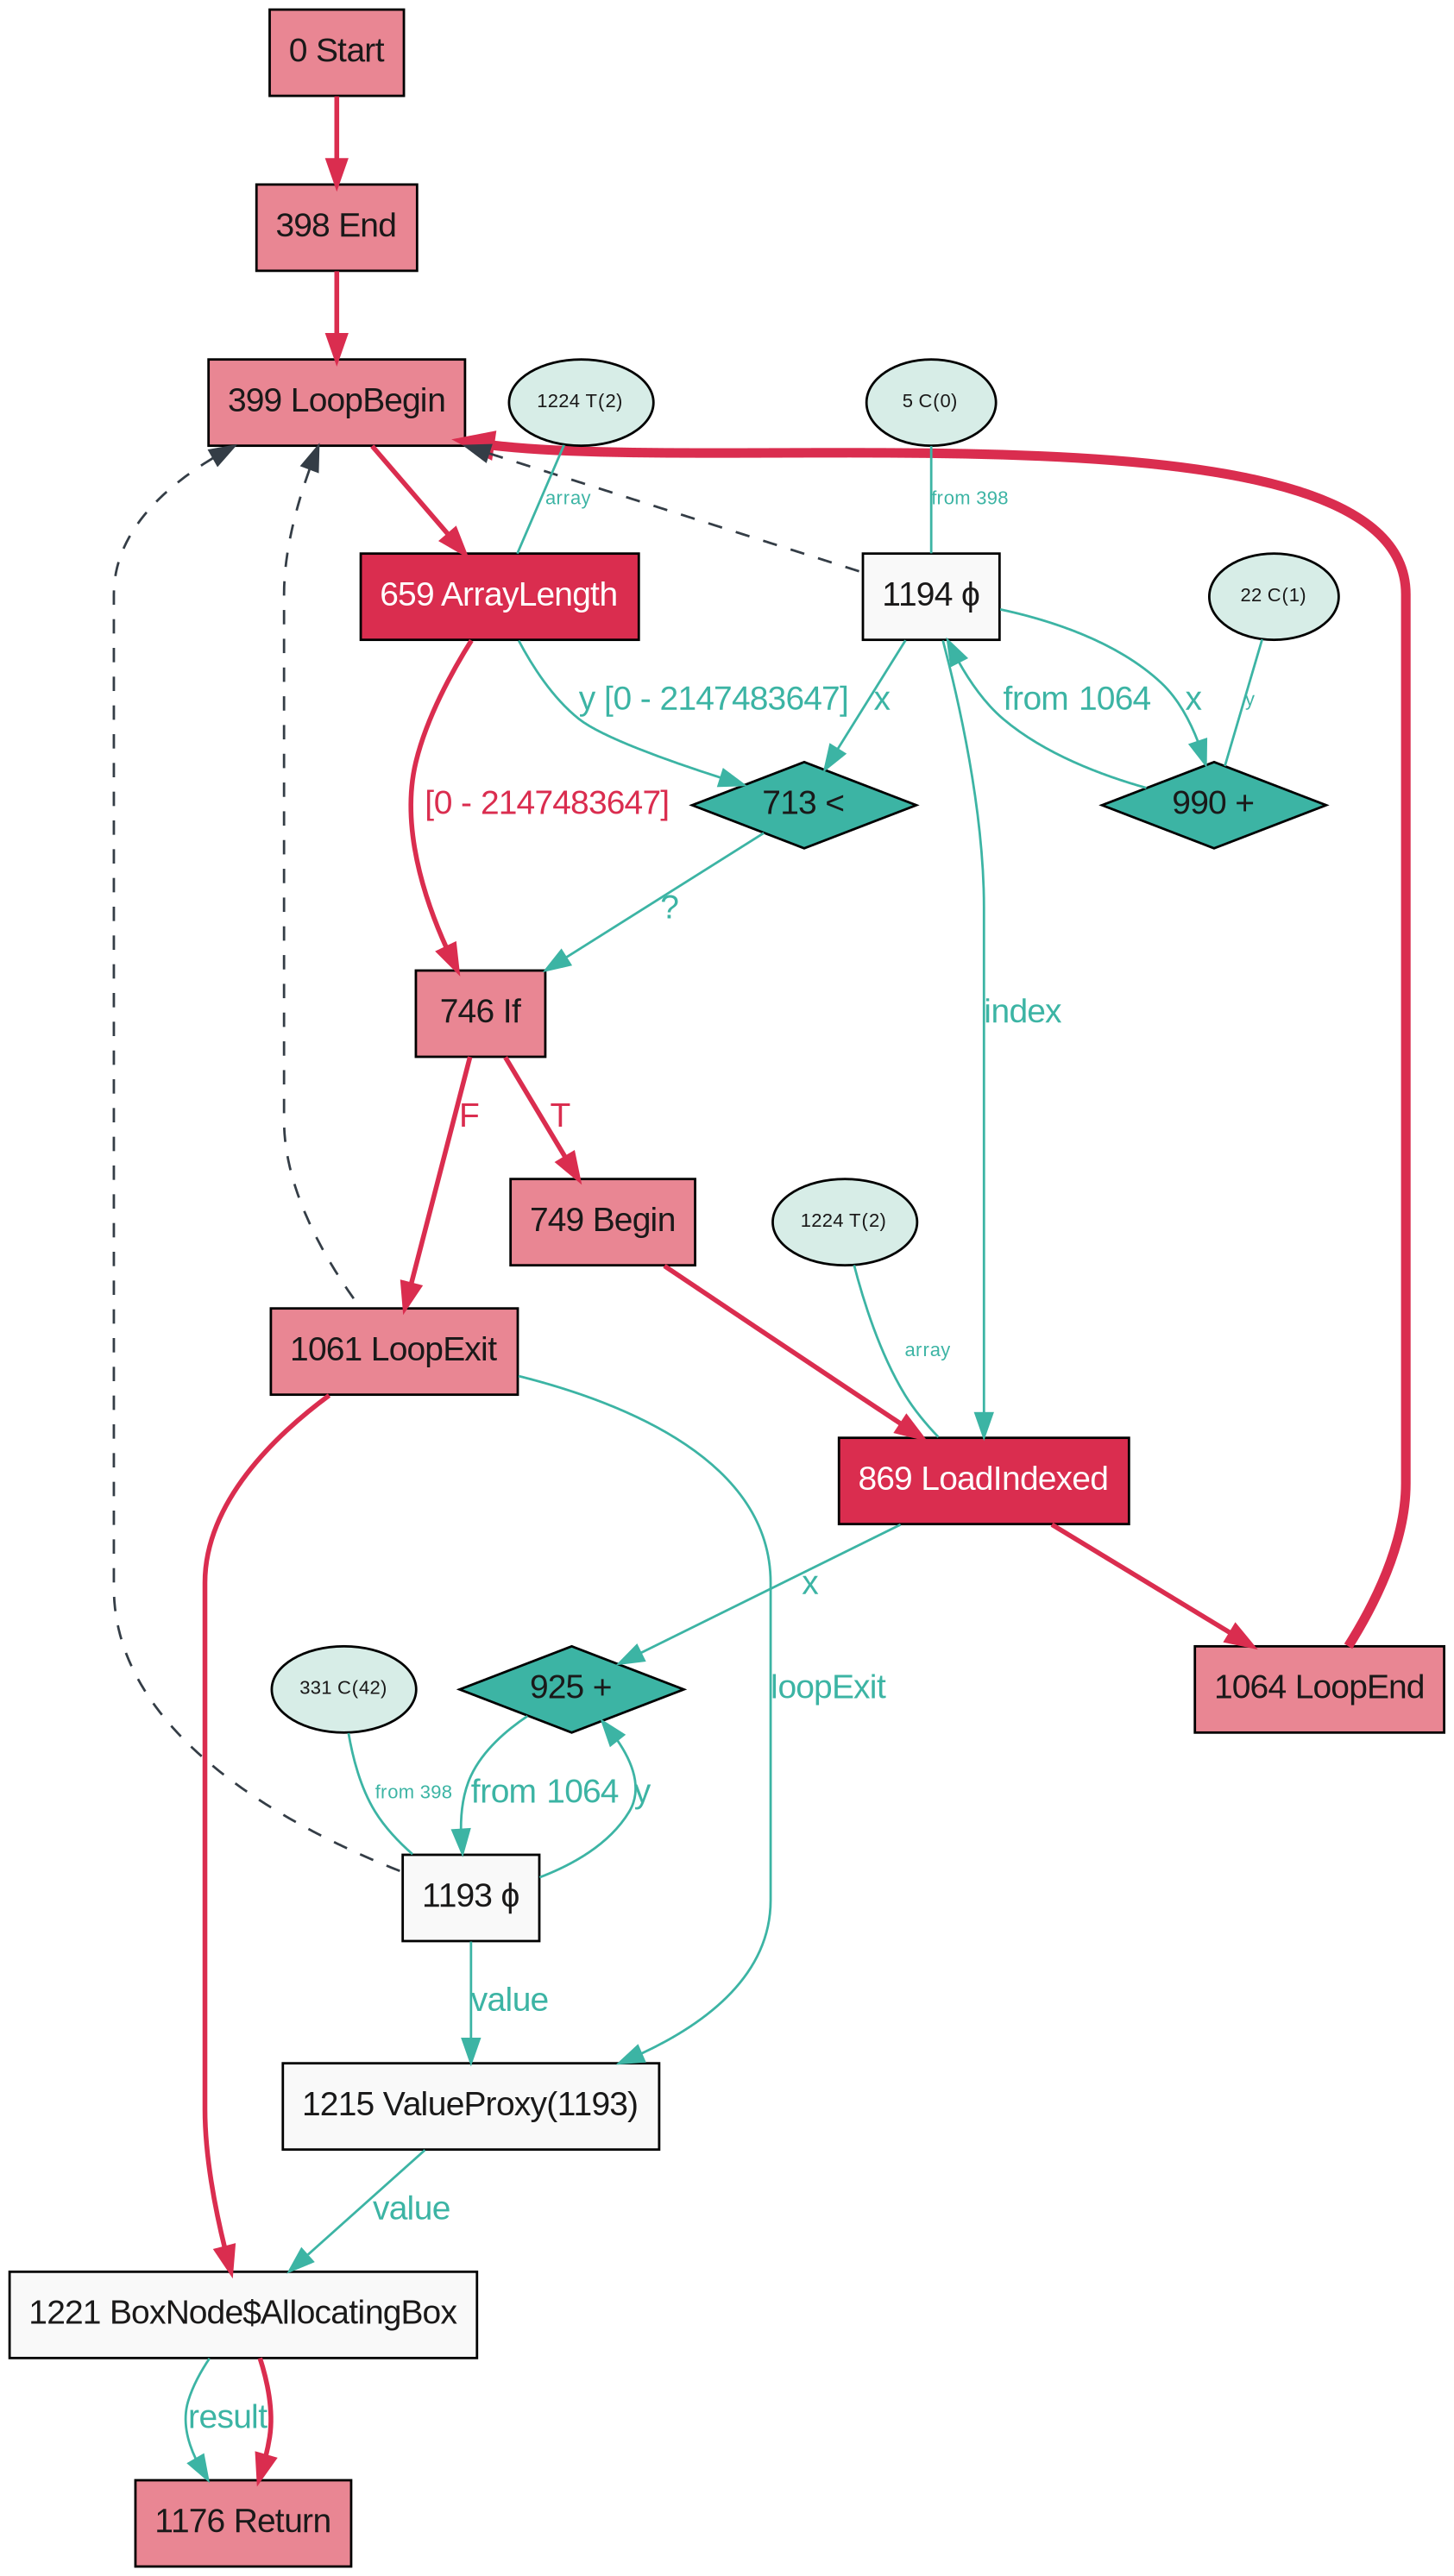
\includegraphics[width=0.5\columnwidth]{figures/checksum:Int:TruffleTier.png}
	\caption{Graal IR graph of specialization \texttt{checksum[Int]} after Truffle tier.}
\end{figure} 